\section{Introduction}\label{sec:Intro}

% Para 1: Stakes — structural alloys matter, development is slow, PSPP space is vast, HEAs compound the problem.

Structural alloys for extreme environments---from ballistic armor to gas turbine blades---underpin performance in defense, aerospace, and energy systems~\cite{pollock2016alloy, reed2006superalloys, arroyave2022perspective}. Although significant advances have been made in computational screening, high-throughput synthesis, and machine learning, the alloy development cycle remains slow and resource-intensive~\cite{liu2022highthroughput}: typically, alloy development programs proceed through iterative synthesis--processing--characterization--testing loops, and each cycle demands reproducibility (i.e., multiple evaluations) across heats, processing routes, and testing protocols. This problem is compounded by the fact that the composition--process--microstructure--performance (PSPP) space over which alloy campaigns operate is vast, and only a minute fraction has been explored directly~\cite{miracle2017critical}. In high-entropy alloy (HEA) systems, where five or more principal elements define a combinatorially large design space, exhaustive exploration is impractical even with advanced experimental methods~\cite{zhang2014microstructures, cantor2004microstructural}.

% Para 2: Science — why HEAs are hard: competing deformation mechanisms, navigable trade-offs, CALPHAD errors at FCC boundaries.

Within this broad landscape, FCC HEAs present a rich but not sufficiently mapped composition--property space. Strength and ductility are governed by competing deformation mechanisms---dislocation glide, twinning, and local chemical ordering---whose relative contributions shift with composition in ways that binary or ternary subsystem data cannot predict. Interaction effects among four or more solutes (i.e., beyond pairwise or ternary interactions) are absent from lower-order assessments, leaving large regions of the compositional space without reliable property estimates. The strength--ductility trade-off, often treated as intrinsic, may instead reflect constrained design trajectories; multi-component spaces can contain regions where twinning-induced plasticity (TWIP), transformation-induced plasticity (TRIP), or both enable simultaneous improvements~\cite{gludovatz2014fracture, li2016metastable, otto2013influences}. Thermodynamic constraints compound the challenge: CALPHAD databases show significant prediction errors at FCC stability boundaries in higher-order systems, and compositions that appear promising from property models frequently form brittle intermetallics. Mapping these composition--structure--property relationships thus requires an exploration strategy that generates both optimized compositions and the physical insight needed to interpret them.

% Para 3: Existing tools — HTP/ICME/ML each fall short. The bottleneck is resource allocation under finite budget.

To date, several distinct frameworks have been applied to this problem. Combinatorial and high-throughput (HTP) approaches, for example, can generate candidate compositions at scale, but open-loop strategies tend to produce a significant fraction of infeasible compositions---alloys with undesired phase constitution---making such campaigns inherently resource-inefficient~\cite{potyrailo2011combinatorial, rajan2008combinatorial}. More targeted campaigns, guided by Integrated Computational Materials Engineering (ICME) models or domain expertise, reduce infeasibility risk but require substantial computational investment and often struggle to integrate multi-scale simulations at acceptable computational cost~\cite{national2008integrated, panchal2013key, arroyave2019systems}. Machine learning (ML) approaches complement these frameworks by enabling rapid screening, yet they frequently defer experimental validation to later stages, particularly for bulk structural alloys where synthesis and testing costs are significant~\cite{yang2022machine}. Despite the progress made, the dominant bottleneck across all these approaches is resource allocation: deciding which chemistries to interrogate under a finite experimental budget~\cite{arroyave2022perspective}.

% Para 4: BO — sequential decision-making under uncertainty. GPs, EHVI, metallurgical priors.

In this context, Bayesian optimization (BO) has rapidly emerged as a principled approach to optimal resource allocation in materials discovery, framing the problem as sequential decision-making under uncertainty~\cite{shahriari2016taking, frazier2018tutorial}. In a BO framework, probabilistic surrogate models (typically Gaussian processes~\cite{Rasmussen:2005:GPM:1162254}) quantify epistemic uncertainty across the design space, and acquisition functions balance (a)~exploration of poorly characterized regions with (b)~exploitation of promising candidates~\cite{snoek2012practical, arroyave2022perspective}. Multi-objective formulations extend this framework to optimize competing performance metrics simultaneously, typically by maximizing the expected hypervolume improvement (EHVI) of the Pareto front~\cite{emmerich2006single, zhao2018fast, mamun2025accelerated, hanaoka2022comparison}. Furthermore, metallurgical knowledge (thermodynamic stability limits, processing windows, and microstructural descriptors) can be encoded directly into surrogate structure and constraint models, improving data efficiency while preserving physical interpretability~\cite{khatamsaz2022multiobjective, vela2023data, paramore2025twoshot}.

% Para 5: Prior art — closed-loop alloy campaigns validate BO in practice (Xue, Rao, Sohail, others).

Over the past decade, closed-loop experimental campaigns that couple BO with iterative alloy synthesis have validated this approach in practice. Xue et al.~\cite{xue2016accelerated} pioneered adaptive alloy design by identifying low-hysteresis NiTi-based shape memory alloys through nine feedback loops exploring fewer than 40 compositions from a space of 800{,}000 candidates. Rao et al.~\cite{rao2022machine} applied iterative ML-guided design to discover high-entropy Invar alloys with near-zero thermal expansion. More recently, Sohail et al.~\cite{sohail2025machine} used domain-knowledge-informed active learning to design FeNiCoAlTa alloys achieving 1.8~GPa yield strength with 25\% elongation. Additional closed-loop campaigns have targeted lead-free solders~\cite{wei2025discovering}, magnesium alloys~\cite{ghorbani2024active}, high-temperature shape memory alloys~\cite{tian2024noise}, and Al--Si alloys~\cite{cai2025process}, with several incorporating multi-objective acquisition strategies~\cite{wei2025discovering, li2022strength}. These studies demonstrate that BO-guided campaigns can identify competitive alloy compositions while exploring less than 1\% of the feasible design space.

% Para 6: Gap — failed experiments waste budget and return no training data. Standard BO ignores feasibility.

However, a practical constraint remains unaddressed in these campaigns: many candidate designs are infeasible and yield no measurable objective values, wasting experimental resources without contributing to surrogate model refinement. We note that in alloy discovery, failure does not indicate poor performance (e.g., low yield strength) but rather that experimental time and resources are expended without obtaining usable measurements---because the alloy cannot be synthesized, processed, or tested under the prescribed conditions. This distinction is consequential: a low-performing alloy still provides training data for the surrogate model, whereas a failed experiment provides none. The cost of each experimental iteration---several thousands of dollars in materials, instrument time, and personnel---means that even a small fraction of failed experiments can substantially reduce campaign efficiency. Yet standard BO frameworks implicitly assume that every queried candidate returns measurable objectives, offering no mechanism to account for experimental viability during candidate selection. \autoref{fig:kkt_schematic} illustrates why this matters: in constrained optimization, the best solutions tend to reside on the feasibility boundary (a consequence of the Karush--Kuhn--Tucker optimality conditions~\cite{nocedal2006numerical}), precisely where the risk of failure is highest. A framework that excludes boundary compositions sacrifices the best candidates; one that ignores feasibility wastes budget on infeasible ones.

\begin{figure}[H]
    \centering
    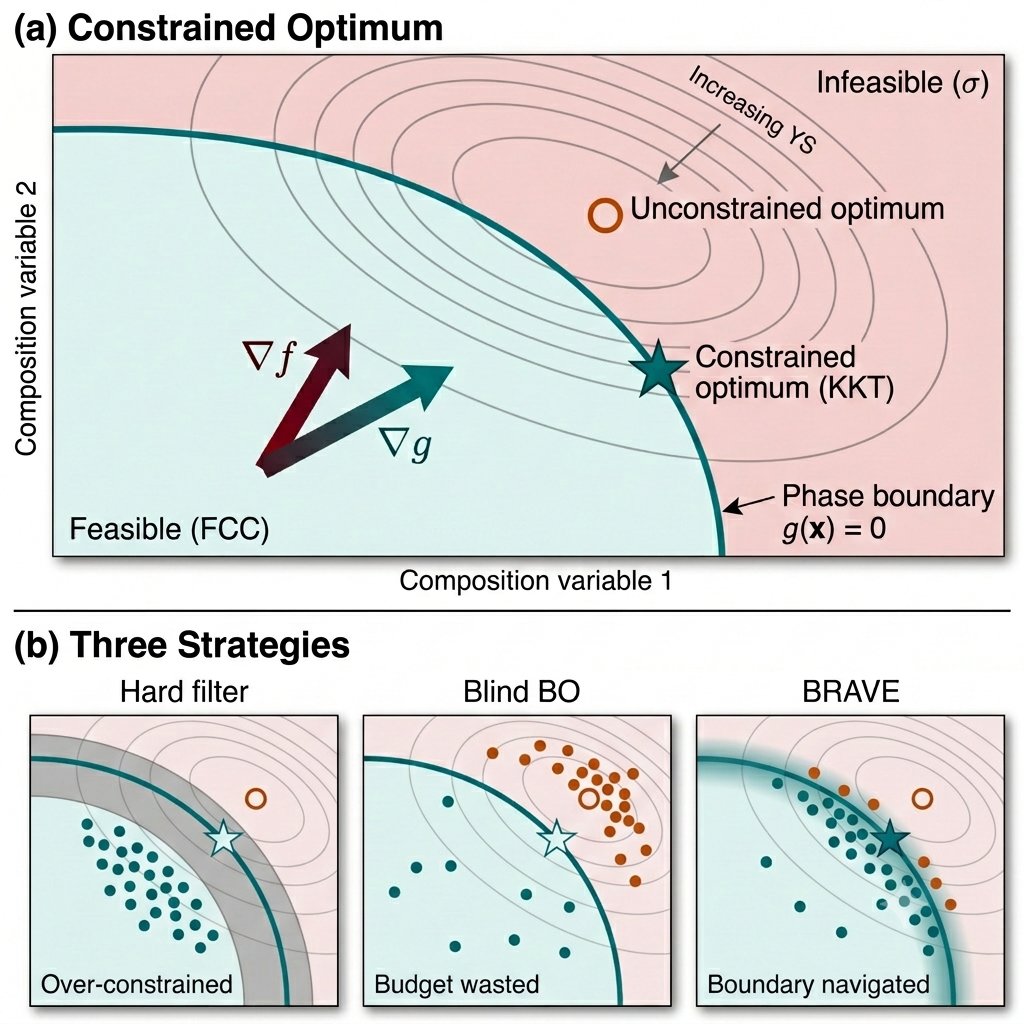
\includegraphics[width=1\columnwidth]{Figures/kkt_boundary_v3_twopanel.png}
    \caption{Constrained optimization in composition space. (a)~When the objective (e.g., yield strength) increases toward the infeasible region (sigma phase), the KKT conditions place the constrained optimum (star) on the phase stability boundary where $\nabla f$ and $\nabla g$ are aligned; the unconstrained optimum (open circle) lies in the infeasible region. (b)~Three acquisition strategies distribute experimental budget differently given the same total number of samples. Hard filtering over-constrains the search by excluding a buffer zone around the boundary, missing the KKT optimum entirely. Feasibility-blind BO concentrates samples near the unconstrained optimum, wasting budget on infeasible compositions. BRAVE navigates the boundary by concentrating samples in the feasible region near the phase stability limit, accepting a small number of infeasible outcomes as the cost of boundary exploration.}
    \label{fig:kkt_schematic}
\end{figure}

% Para 7: Gap sharpened — constraint-aware BO spreading across domains; alloys lack experimental deployment.

Constraint-aware acquisition strategies have begun to address this gap across several domains. Hickman et al.~\cite{hickman2025anubis} introduced feasibility-aware acquisition functions that reduce failed experiments in perovskite and drug synthesis. Low et al.~\cite{low2024evolution} developed evolution-guided constrained optimization for self-driving chemistry laboratories. Chen et al.~\cite{chen2026materials} coupled constrained expected improvement with representation learning for computational catalyst and transparent conductor design. Tamura et al.~\cite{tamura2023nims} integrated feasibility constraints into autonomous robotic materials exploration. In alloy systems specifically, constraint-aware formulations have been proposed~\cite{khatamsaz2022multiobjective, khatamsaz2023bayesian}, and physics-informed feasibility classifiers have been developed~\cite{hardcastle2025physics}, but no experimental alloy campaign has yet integrated a learned feasibility model directly into the multi-objective acquisition function within an iterative workflow.

% Para 8: BIRDSHOT + Campaign 1 — what it achieved, what it couldn't handle (sigma phases, no failure mechanism).

The BIRDSHOT (Batch-wise Improvement in Reduced Design Space using a Holistic Optimization Technique) framework was developed to integrate computational screening, high-throughput experimentation, and batch Bayesian optimization within an iterative design--make--test--learn workflow~\cite{mulukutla2024illustrating, hastings2025accelerated} (\autoref{fig:birdshot_framework}).

\begin{figure}[H]
    \centering
    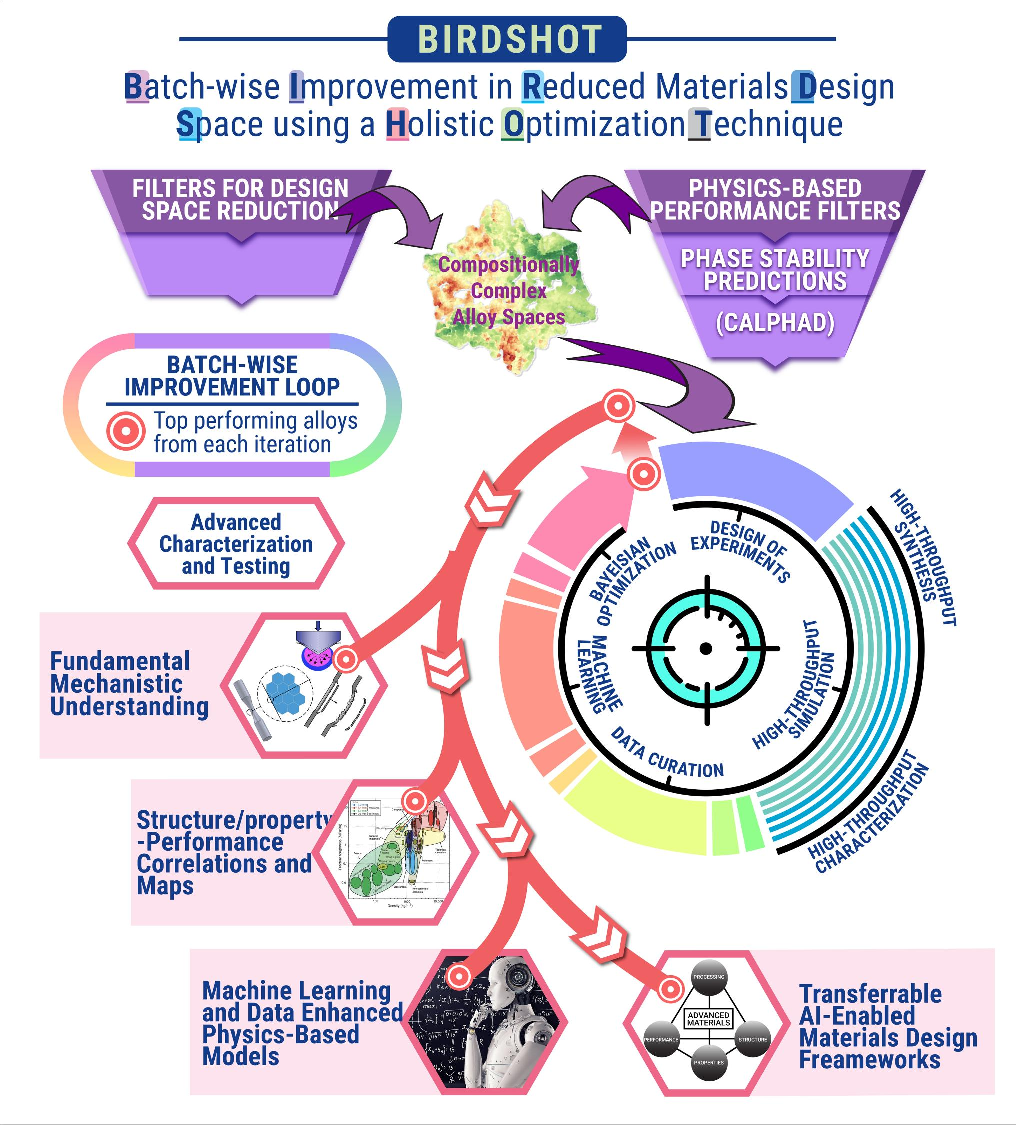
\includegraphics[width=1\columnwidth]{Figures/birdshot_framework.pdf}
    \caption{Overview of the BIRDSHOT framework. Physics-based filters (CALPHAD phase stability, property constraints) reduce the design space before optimization begins. The iterative loop cycles through design of experiments, high-throughput simulation, high-throughput characterization, data curation, and machine learning, with Bayesian optimization closing the loop at each iteration. Reproduced from:~\cite{hastings2025accelerated}.}
    \label{fig:birdshot_framework}
\end{figure}

In a prior campaign, we applied BIRDSHOT to the six-component Al--V--Cr--Fe--Co--Ni FCC HEA system, targeting three mechanical objectives (UTS/YS ratio, hardness, and strain rate sensitivity) under four constraints (single-phase FCC at 700$^\circ$C, density $<$ 8.5~g/cm$^3$, thermal conductivity $>$ 5~W/(K$\cdot$m), and SFE regime classification)~\cite{hastings2025accelerated}. Five iterative design--make--test--learn loops, each synthesizing 8 alloys via vacuum arc melting, identified Pareto-optimal compositions by exploring only 0.15\% of the feasible design space. That campaign established the viability of iterative, multi-objective Bayesian optimization for structural alloy development. Although successful in identifying Pareto-optimal compositions, it also exposed limitations. CALPHAD phase stability predictions were imperfect: several alloys predicted to be single-phase FCC showed sigma or BCC secondary phases. The framework had no mechanism to account for these failed experiments, which consumed resources without contributing to model refinement. A detailed summary of this earlier work is provided in the Supplemental Information.

% Para 9: Transition — three extensions.

In the present work, we report a second discovery campaign that extends the BIRDSHOT framework in three directions, addressing the limitations identified above. The campaign also exposes a tension inherent to this alloy system: vanadium, the dominant strengthening solute, simultaneously promotes sigma-phase formation, forcing the best alloys onto the FCC phase stability boundary where the risk of experimental failure is highest.

% Para 10: Extension 1 — BRAVE: risk-aware acquisition via GP feasibility classifier on EHVI.

First, we introduce a risk-aware acquisition strategy---Bayesian Risk-Aware Alloy Discovery and Exploration (BRAVE)---that penalizes candidates likely to produce failed experiments (i.e., alloys that form secondary phases and yield no usable objective data). Alloys predicted to form single-phase FCC structures but found to contain secondary phases are classified as failures: they introduce processing challenges and do not provide a consistent basis for comparison within the intended single-phase design space. To mitigate this risk, we extend the EHVI acquisition function with a learned Gaussian process classifier that estimates the probability of experimental viability for each candidate composition. High-risk candidates receive a probabilistic penalty during acquisition scoring, reducing their selection priority. We note that \emph{the penalty is soft}: a candidate with sufficiently high predicted objective values can still be selected despite elevated risk, preserving controlled exploration in uncertain but potentially high-performing regions.

% Para 11: Extension 2 — 8-element space (Mn for SFE/twinning, Cu for solubility limits), diversity sampling.

Second, we expand the design space from the previous 6-element system to an 8-element system, Al--V--Cr--Mn--Fe--Co--Ni--Cu. The inclusion of Mn and Cu introduces additional degrees of freedom for tuning ductility and phase stability, guided by prior experimental insights and domain knowledge. Mn is expected to reduce the stacking fault energy in FCC alloys, potentially promoting mechanical twinning and enhancing strain-hardening capacity. Cu expands the accessible composition space but has positive mixing enthalpies with Fe, Co, and Cr, driving FCC phase separation into Cu-rich and Cu-lean regions and creating thermodynamic boundaries that test the limits of current CALPHAD predictions. Grid sampling at 4~at.\% resolution yields approximately 3.4 million candidate compositions, of which $\sim$27{,}000 (i.e., less than 1\%) are predicted to form single-phase FCC structures after CALPHAD screening. To enable tractable exploration of this feasible space, we use a diversity-aware sampling strategy based on k-medoids clustering~\cite{paramore2025twoshot} across 37 chemically distinct subsystems. This prioritizes compositionally informative candidates over redundant clusters, improving early-stage surrogate learning through better coverage of the design space.

% Para 12: Extension 3 — five objectives as multi-scale deformation probes; DoP as simulation-in-the-loop.

Third, five objectives are evaluated through a coordinated high-throughput characterization workflow: yield strength (YS), UTS/YS ratio, strain at UTS, dynamic-to-quasi-static hardness ratio ($H_\text{dyn}/H_\text{qs}$), and depth of penetration (DoP). These objectives serve as complementary probes of deformation behavior across strain rates, spanning (a)~quasi-static tensile response, (b)~rate-dependent behavior measured by nanoindentation and split Hopkinson pressure bar (SHPB) testing, and (c)~simulated impact resistance computed via finite-element modeling. Among these, DoP is derived from ballistic impact simulations parameterized by Cowper--Symonds constitutive models calibrated to the quasi-static tensile and dynamic SHPB data acquired within each iteration. This creates a simulation-in-the-loop architecture in which experimental measurements from one stage of characterization feed directly into a computational objective evaluated within the same design cycle, coupling experiment and simulation within a single design iteration.

% Para 13: Roadmap — figure reference, what the paper delivers.

The complete BIRDSHOT framework---encompassing computational design, synthesis, characterization, and simulation---is summarized in \autoref{fig:full_framework}. By addressing thermodynamic constraints, manufacturability, and experimental throughput within a closed-loop workflow, this campaign demonstrates risk-aware, multi-objective optimization through three iterative experimental cycles. The remainder of this paper presents the design methodology, experimental results across three closed-loop iterations, and the implications for feasibility-aware optimization in high-dimensional compositional spaces.

\begin{figure*}[t]
    \centering
    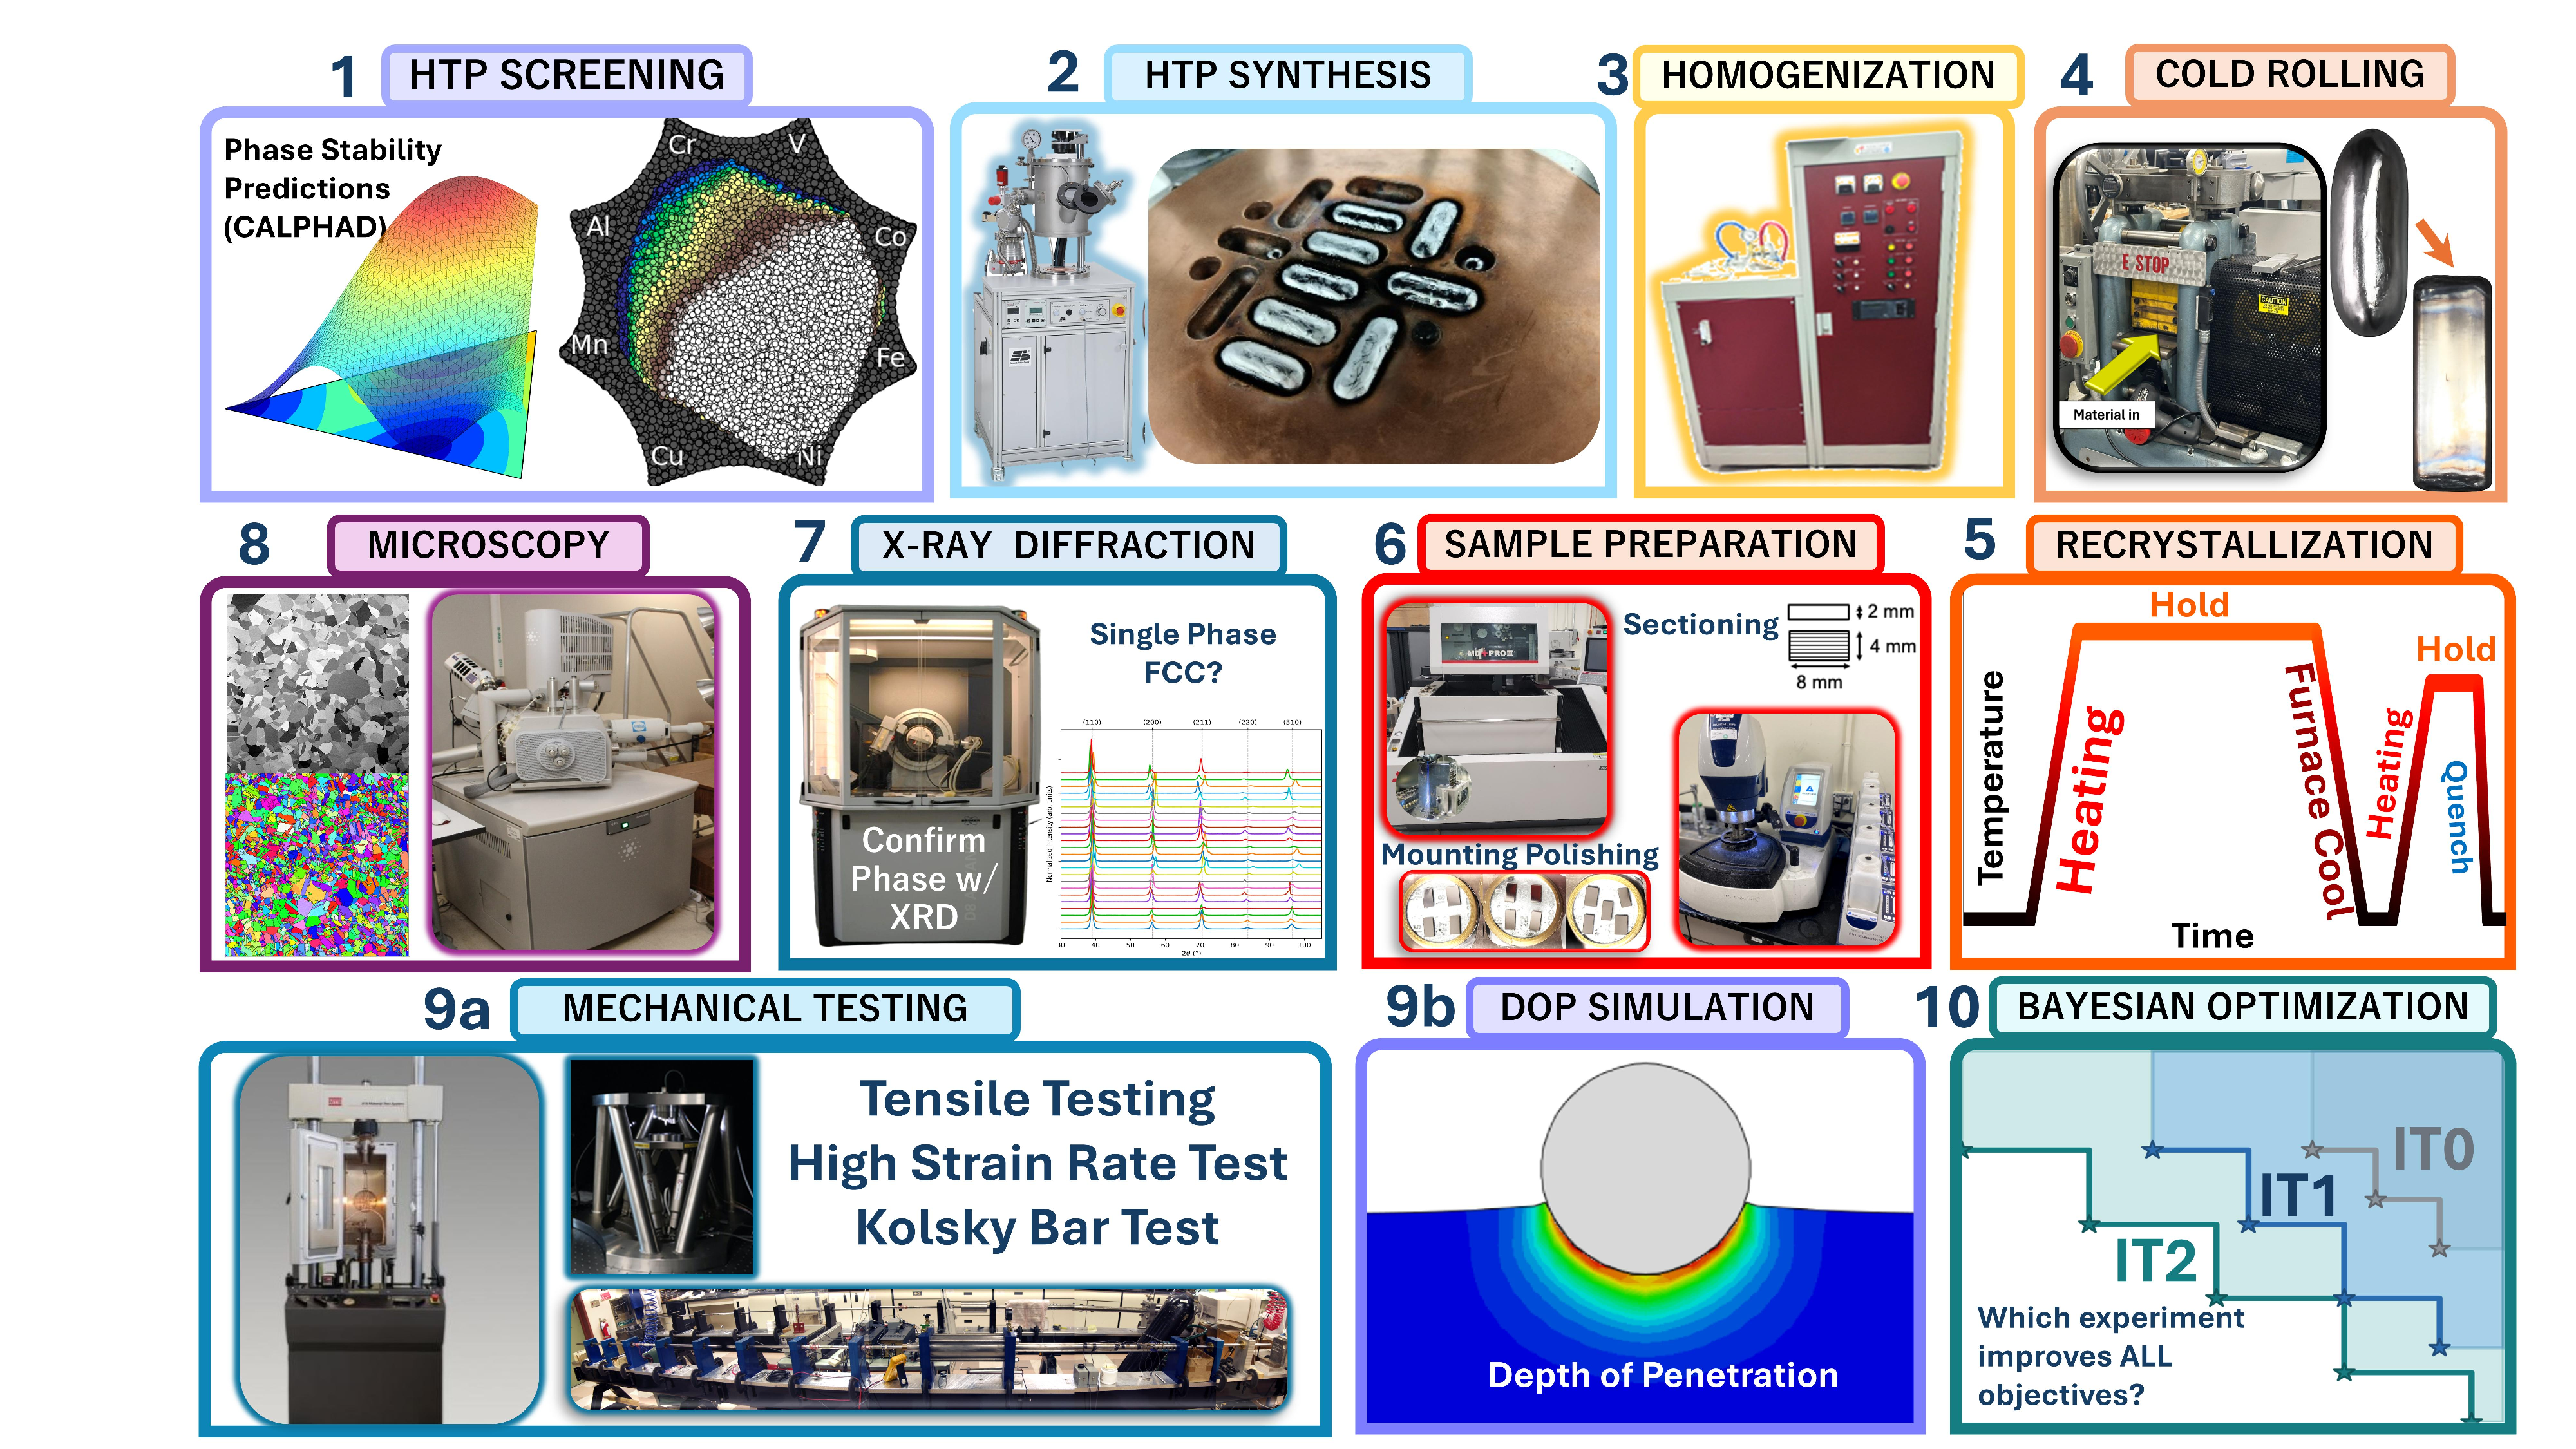
\includegraphics[width=1\textwidth]{Figures/C2_Schematic.pdf}
    \caption{BIRDSHOT workflow from computational design through synthesis, characterization, and simulation. The iterative loop feeds experimental measurements and phase verification results back into the Bayesian optimization framework, which updates surrogate models and the feasibility classifier before selecting the next batch of candidate alloys.}
    \label{fig:full_framework}
\end{figure*}
